\chapter{Computationally-Efficient Learning}
\label{ch:10-efficient-learning}

\lecturemeta{Dan Alistarh}{ISTA}

Alistarh opens with the bitter lesson, that general methods leveraging computation win by a large
margin, and then turns it against itself. If computation is the scarce resource, the discipline
of making methods computationally efficient is not opposed to the bitter lesson but is its
consequence, which he later names the bitter lesson squared: designing computationally efficient
methods to make large models more computationally efficient. The evidence for scarcity is a
scissors between demand and supply, and the rest of the lecture is one mathematical idea applied
to closing it. That idea is that quantization error should be measured in loss space rather than
weight space, weighted by the inverse Hessian, which turns out to be a 1990 result rediscovered
at scale.

\section*{Key ideas}

\paragraph{The gap, in three numbers.} Between 2020 and 2025, on public data, computation used to
train state-of-the-art models rose by roughly 50,000 times and inference computation by roughly
300 times, while the capability of the best available GPU rose by only about 20
(Figure~\ref{fig:efficient-learning-1}). The slide labels the resulting divergence a 2500-fold gap.
Since hardware is visibly not closing it, algorithms must, and the concrete stakes are given in
model sizes: Llama-4 Maverick at 400 billion total parameters, 800 GB at half precision, 17
billion active across 128 experts, trained on 22 trillion tokens for about 6 million GPU hours.
The lecture also puts a cost on inference rather than training, quoting a Google study from
August 2025: a median generative query consumes 0.24 Wh, 0.03 g of CO$_2$e, described as nine
seconds of television, and 0.26 mL of water, five drops. The caveats are given honestly, that
medians hide heavy prompts and that market-based carbon accounting undercounts location-based.

\begin{figure}[htbp]
\centering
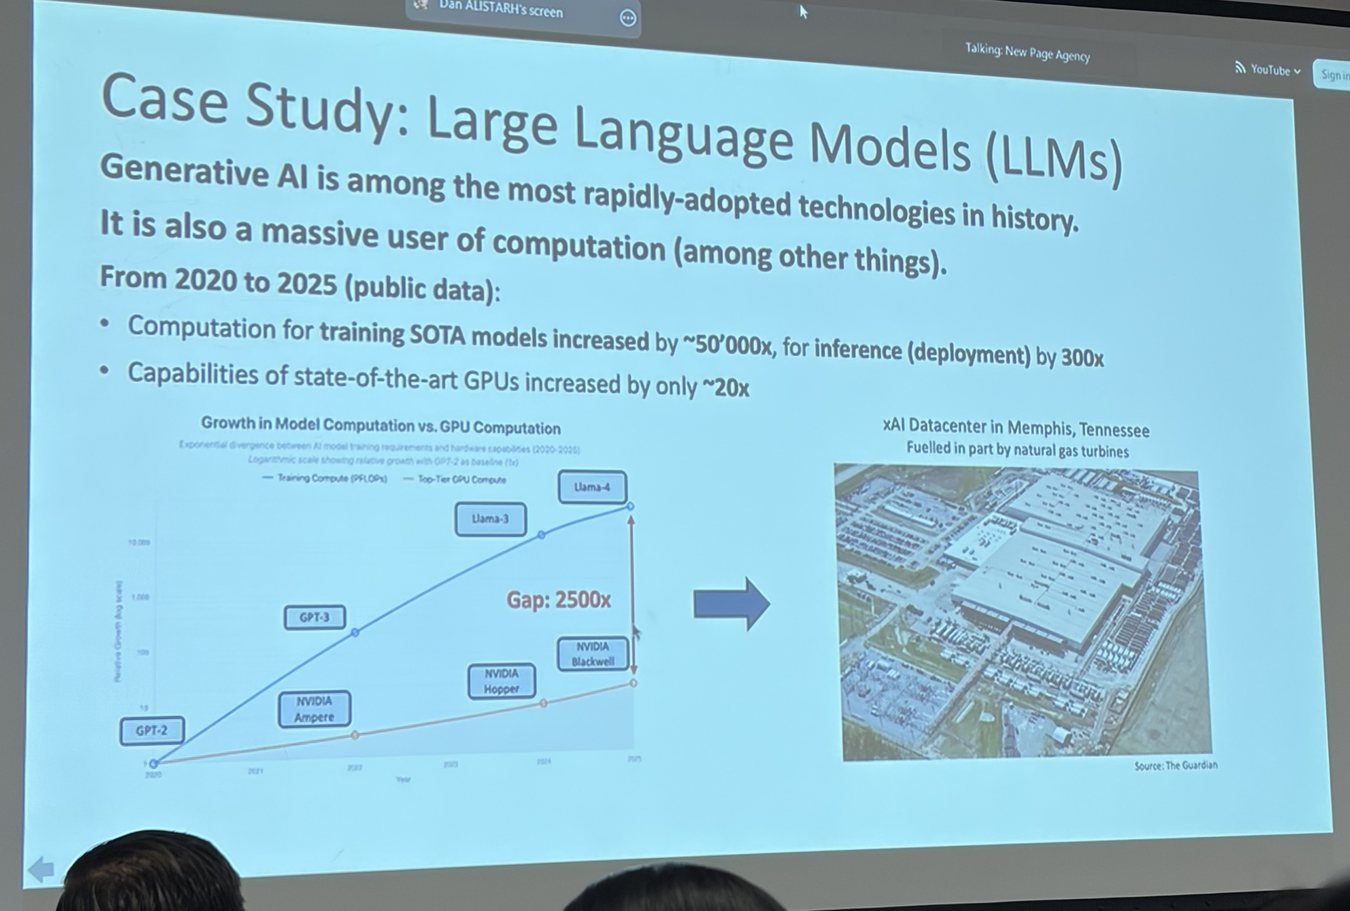
\includegraphics[width=0.86\textwidth]{figures/efficient-learning-1.jpg}
\caption{The argument for the whole lecture, from the Computationally-Efficient Learning slides,
photographed during the talk. Training compute per state-of-the-art model and top-tier GPU
capability are plotted on a log scale with GPT-2 as baseline. The two curves diverge from GPT-2
through GPT-3 to Llama-3 and Llama-4 while the hardware line stays nearly flat across Ampere,
Hopper and Blackwell, leaving the annotated 2500-fold gap. The photograph on the right is the xAI
data centre in Memphis, partly gas-fuelled.}
\label{fig:efficient-learning-1}
\end{figure}

\paragraph{The mathematics is about the loss, not the weights.} This is the load-bearing
derivation and it is short. Quantization is just a particular weight perturbation,
$\mathrm{Compress}(\wt) = \wt + \dw$. Taylor expanding the loss,
\[
  \Loss(\wt + \dw) \approx \Loss(\wt) + \grad_{\wt}\Loss \cdot \dw
    + \tfrac{1}{2}\,\dw\T \Hess\, \dw,
\]
\noindent and since the weights are trained, $\grad_{\wt}\Loss \approx \vect{0}$, so the quantity
actually being minimised is the quadratic form $\tfrac12 \dw\T \Hess \dw$ subject to $\dw$ having
the admissible form $\delta w_i = w_i - \quant(w_i)$ for quantizer $\quant$. For a single weight
the optimum is
\[
  \text{LossImpact}(w_i) = \frac{\bigl(w_i - \quant(w_i)\bigr)^2}{2\,[\Hess\inv]_{ii}},
  \qquad
  \dw^{*} = -\,\frac{w_i - \quant(w_i)}{[\Hess\inv]_{ii}}\; \Hess\inv_{:,i}.
\]
\noindent Two things follow. The cost of rounding a weight is not its rounding error but that
error divided by the corresponding inverse-Hessian entry, so weights differ enormously in how much
they may be moved. And the correction $\dw^{*}$ spreads compensation across the other weights,
which is why good quantizers adjust what they have not yet touched. The lecture attributes this
lineage explicitly to Optimal Brain Damage and Optimal Brain Surgeon, from 1990 and
1993~\citep{lecun1990, hassibi1993}, and to its own scaling in the Optimal Brain Compressor.

\paragraph{Why it becomes practical at LLM scale.} GPTQ and SparseGPT minimise a layer-wise loss
$\norm{\mat{Y}_\ell - \mat{X}_\ell \est{\mat{W}}_\ell}^2$ whose Hessian is
$\mat{X}_\ell \mat{X}_\ell\T$, and the observation that unlocks everything is that this Hessian is
constant with respect to the weights, so it can be precomputed once at the start of
compression~\citep{frantar2023gptq, frantar2023sparsegpt}. The algorithm then sweeps columns of
$\mat{W}_\ell$: quantize column $j$ in saliency order within a block, compute the error, and
update the columns to the right of $j$ using $\dw^{*}$. The supporting machinery is a family of
linear time and space estimators of second-order information at block, layer and global
granularity, with the observation that different models need different granularities.

\paragraph{What the large study actually found.} A million-plus individual task and model
evaluations~\citep{kurtic2025} yield three findings the lecture reduces to one slide. Eight-bit
quantization is essentially lossless. All compression approaches land within roughly 1\% of
baseline on easy benchmarks but degrade more on harder ones, reasoning in particular. And larger
models, 70B and above, are easier to compress and compress more stably across tasks. The study
deliberately restricted itself to schemes with hardware support, W4A16 with INT4 and W8A8 dynamic
per-token with INT8 and FP8, which is what makes the numbers actionable rather than academic.

\paragraph{From measurement to prediction.} The last technical move is to stop measuring the damage
and predict it. The linearity theorem claims that under stated assumptions the effect of
quantization on perplexity is approximately linear in the relative layer-wise squared error,
\[
  \Ex\bigl[\PPL(\est{\mat{W}})\bigr] \approx \PPL(\mat{W}^{*})
    + \sum_{\ell=1}^{L} \alpha_\ell\, t_\ell^{2},
\]
\noindent with $\alpha_\ell$ absolute per-layer constants and $t_\ell$ the $L_2$ error at layer
$\ell$~\citep{malinovskii2025}. The disclaimer is stated on the slide rather than buried: the
theory holds only for methods that do not update weights, so it covers AWQ but not GPTQ. That is a
real limitation, since GPTQ's whole mechanism is the compensating update.

\section*{Notation}

$\wt$ are trained weights, $\dw$ the quantization perturbation, $\quant$ the quantizer, $\Hess$
the Hessian and $\PPL$ perplexity. Note that $\Hess$ here is a Hessian, whereas $\Hcent$ in
Chapter~\ref{ch:02-representational-geometry} is a centring matrix, and the two are kept visually
distinct for exactly that reason.

\section*{Why it matters}

This chapter pairs with the summer school's quantization tutorial, which implements
round-to-nearest and GPTQ against the same mathematics and exhibits the 4-bit failure the findings
predict. It also converges
with Pascanu (Chapter~\ref{ch:07-to-be-figured-out}) on the same diagnosis from a different
direction: Pascanu profiles memory bandwidth and concludes the recurrent block should be cheap,
Alistarh reduces bit-width so the weights fit in faster memory, and both are treating arithmetic
as abundant and data movement as scarce. The lottery ticket citation is shared with
Chapter~\ref{ch:01-intro-deep-learning} under a different interpretation, which is noted there.

\begin{aside}
The framing device deserves attention independently of the content. Alistarh takes the bitter
lesson, which is normally deployed as an argument against clever methods, and derives from it a
mandate for clever methods, on the grounds that if compute is what matters then compute
efficiency is what matters. The move is available whenever a scaling argument is used to dismiss
an idea: ask what the argument implies about the price of the resource it says is decisive.
\end{aside}
